\documentclass[italian]{article}
\usepackage[italian]{babel}
\usepackage{authblk}
\usepackage{hyperref}
\usepackage{graphicx}

\renewcommand\Authand{ e }

\title{Trasporto ferroviario e Open Data\\\small{in \textit{non meno}
        di una e \textit{non più} di quattro pagine}}
\date{\textsc{Anno Accademico 2022-2023}}

\author[1]{Marco Aceti}

\author[2]{Andrea Trentini}

\affil[1]{\small{Laureando, matr.\@ 963032}}

\affil[2]{\small{Relatore}}

\begin{document}
\maketitle

\begin{abstract}
    In Italia non esistono Open Data sulle \textit{performance} del
    trasporto pubblico ferroviario: le metriche definite nei contratti
    di servizio tra gli enti locali committenti e le imprese
    ferroviarie sono insufficienti e spesso inaccessibili.  Il lavoro
    di Tesi si articola sull'idea di preservare i dati istantanei
    della circolazione ferroviaria dalla piattaforma ViaggiaTreno per
    produrre dataset storici, \textit{machine-readable} e di qualità.
    Infine, si propone un'analisi dei dati raccolti a fini statistici
    e di verifica.
\end{abstract}

\section{Introduzione}

In Italia il servizio di trasporto pubblico è operato da
aziende\footnote{\url{https://it.wikipedia.org/wiki/Aziende_di_trasporto_pubblico_italiane}}
private o partecipate.  Sul territorio nazionale sono
autorizzate\footnote{\url{https://www.mit.gov.it/documentazione/elenco-imprese-ferroviarie-titolari-di-licenza-1}}
una ventina di \textit{Imprese Ferroviarie} (IF) adibite al trasporto
passeggeri aventi in essere numerosi \textit{Contratti di Servizio}
(CdS) con gli enti locali (tipicamente le Regioni).  La valutazione
della qualità del servizio è tipicamente affidata agli enti
committenti tramite complessi meccanismi di penali e metriche.

La qualità del servizio è misurata da \textbf{metriche di
    \textit{performance}} stabilite nei CdS e comunicate agli enti
dalle IF\@.  Le suddette metriche non sono affatto sufficienti per
un'\textbf{analisi completa} e \textbf{approfondita}.  Ad esempio, i
dati pubblicati da Regione Lombardia in
\figurename~\ref{lombardia_puntualita} non sono aggiornati da oltre un
anno, sono in formato PDF, sono \textit{brutalmente} aggregati per
mese e non considerano le fermate intermedie o ritardi superiori a 5
minuti.  È apparsa fin da subito evidente la necessità di lavorare sui
\textbf{dati grezzi}, \textit{scrapabili} dalle API di Viaggiatreno e
Trenord.

\begin{figure}[t] \centering
    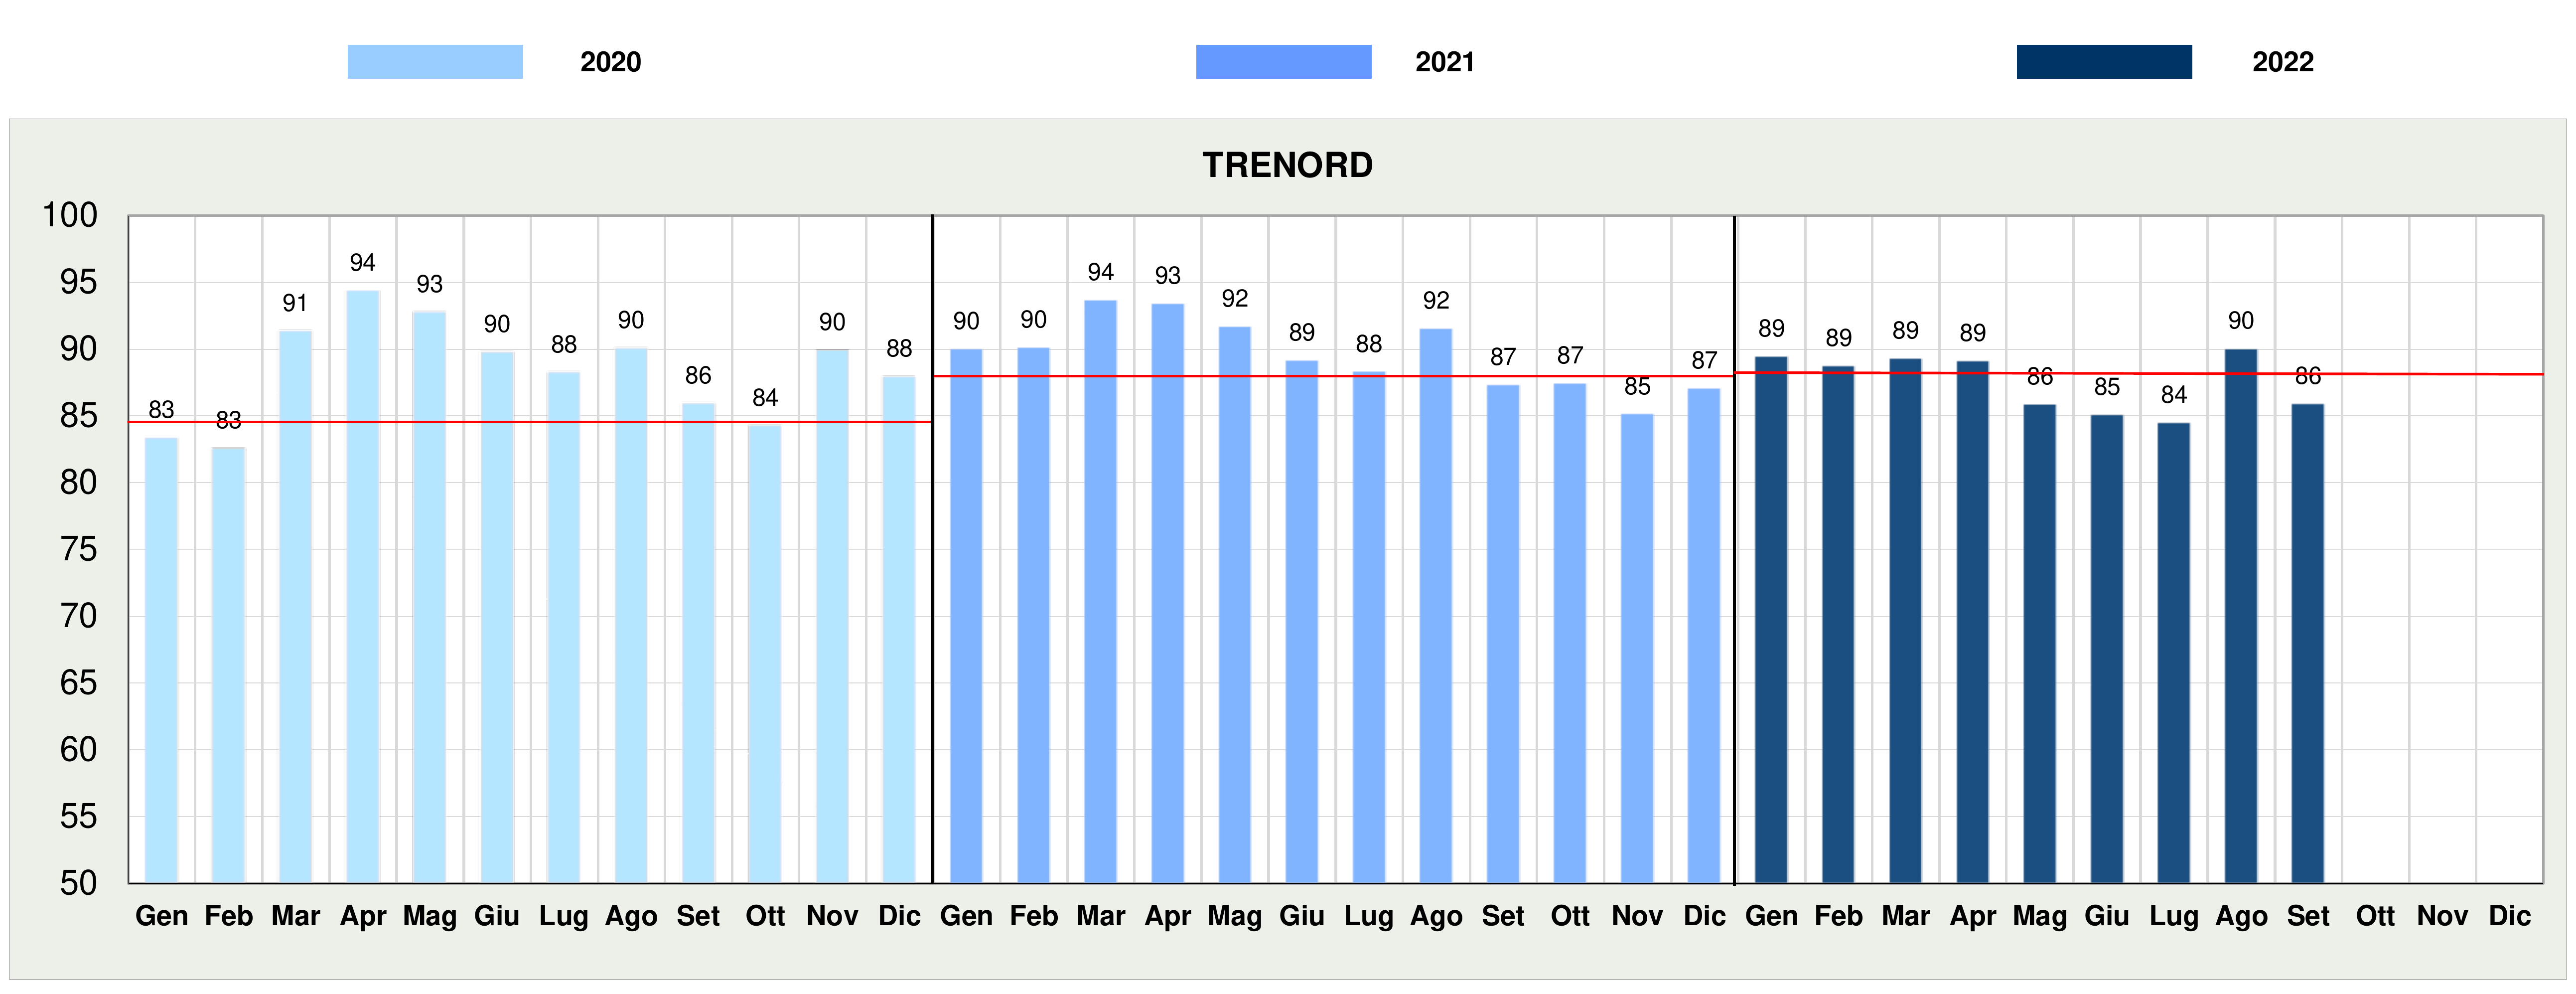
\includegraphics[width=1\textwidth]{images/lombardia_puntualita.png}
	\caption{Dati ufficiali sulla puntualità dei treni in Lombardia:
        percentuale di treni arrivati a destino con al più di 5
        minuti, escludendo cause esterne, lavori programmati e scioperi}
    \label{lombardia_puntualita}
\end{figure}

\subsection*{Panorama giuridico, politico e legislativo}

Durante il lavoro di Tesi è stato fatto ampio uso delle informazioni
fornite dalle API del portale Viaggiatreno, senza aver chiesto alcuna
autorizzazione a Trenitalia o al Gruppo Ferrovie dello Stato Italiane.
Non è però affatto scontato che i dati del trasporto \textit{pubblico}
--- come gli orari dei treni --- siano \textbf{riproducibili} e
\textbf{distribuibili} senza licenza.  Le \textit{note legali} del
portale Viaggiatreno vietano infatti l'uso dei dati per fini diversi
da quelli personali.

Nel 2019 Trenìt, nota applicazione Android e iOS che permette di
confrontare le tariffe ferroviarie, è stata \textbf{citata in
    giudizio} da Trenitalia per questa ragione.  Nonostante abbia
vinto la causa, il dibattito resta aperto.  Il lavoro di Tesi è
comunque tutelato dalle eccezioni alla Legge sul diritto d'autore per
le attività di ricerca scientifica non a fini di lucro.

L'Autore ha inoltre inoltrato due istanze di \textbf{accesso civico
    generalizzato} al fine di accedere ai dati detenuti dalle
Enti Committenti, con parziale successo.

\section{Progettazione e implementazione}

Il software è caratterizzato da tre moduli: lo \textit{scraper},
l'\textit{extractor} e l'\textit{analyzer}.  Il primo si occupa di
scaricare con un \textbf{algoritmo di salvataggio incrementale} le
informazioni \textit{real-time} sulla circolazione ferroviaria, il
secondo \textbf{converte} quanto salvato in comodi file CSV e l'ultimo
propone delle \textbf{analisi predefinite}.  Tutti gli strumenti sono
scritti in Python, sono \textit{open-source} e sono utilizzabili da
CLI\footnote{\textit{Commad Line Interface}, interfaccia a linea di comando}.

Le API, puntualmente documentate nell'Elaborato in \S~A.1, presentano
\textbf{numerose incongruenze e criticità}.  La progettazione ha
dovuto gestire, tra le altre cose, l'assenza di identificatori univoci
affidabili, risorse duplicate, \textit{timestamp} invalidi e
incogruenze tra i dati di Trenitalia e Trenord.  A fini di
performance, è stata implementata una \textbf{\textit{cache}
    associativa} per le informazioni sulle stazioni invarianti nel
tempo.

Un'altra sfida è stata definire programmaticamente il concetto di
\textbf{linea/direttrice ferroviaria}.  Nell'Elaborato (\S~2.4.1) è
stata proposta una \textbf{definizione puntuale} utilizzata nelle
analisi successive.

L'\textit{analyzer} supporta \textbf{filtri} per intervallo di date,
imprese e linee ferroviarie.  È inoltre possibile \textbf{raggruppare}
il \textit{dataset} per treno, impresa ferroviaria o giorno della
settimana ed eventualmente \textbf{riaggreggare} con funzioni come
\textit{media} o \textit{ultimo}.

\section{Analisi e risultati}

Dal \textbf{1° aprile 2023} al \textbf{31 agosto 2023} sono state
raccolte oltre $\sim 10^7$ \textbf{eventi fermata-treno} aventi un
\textbf{ritardo medio} in arrivo di 2.81 minuti e in partenza di 3.99
minuti.

L'\textit{analyzer} supporta alcune \textbf{statistiche predefinite}
parametrizzabili a discrezione dell'utente.  L'obiettivo è stato
fornire un'interfaccia semplice per poter generare visualizzazioni
\textbf{riproducibili}, come quella mostrata in Figura~\ref{figure:delay_box_rc}.

\begin{figure}[h]
    \centering
    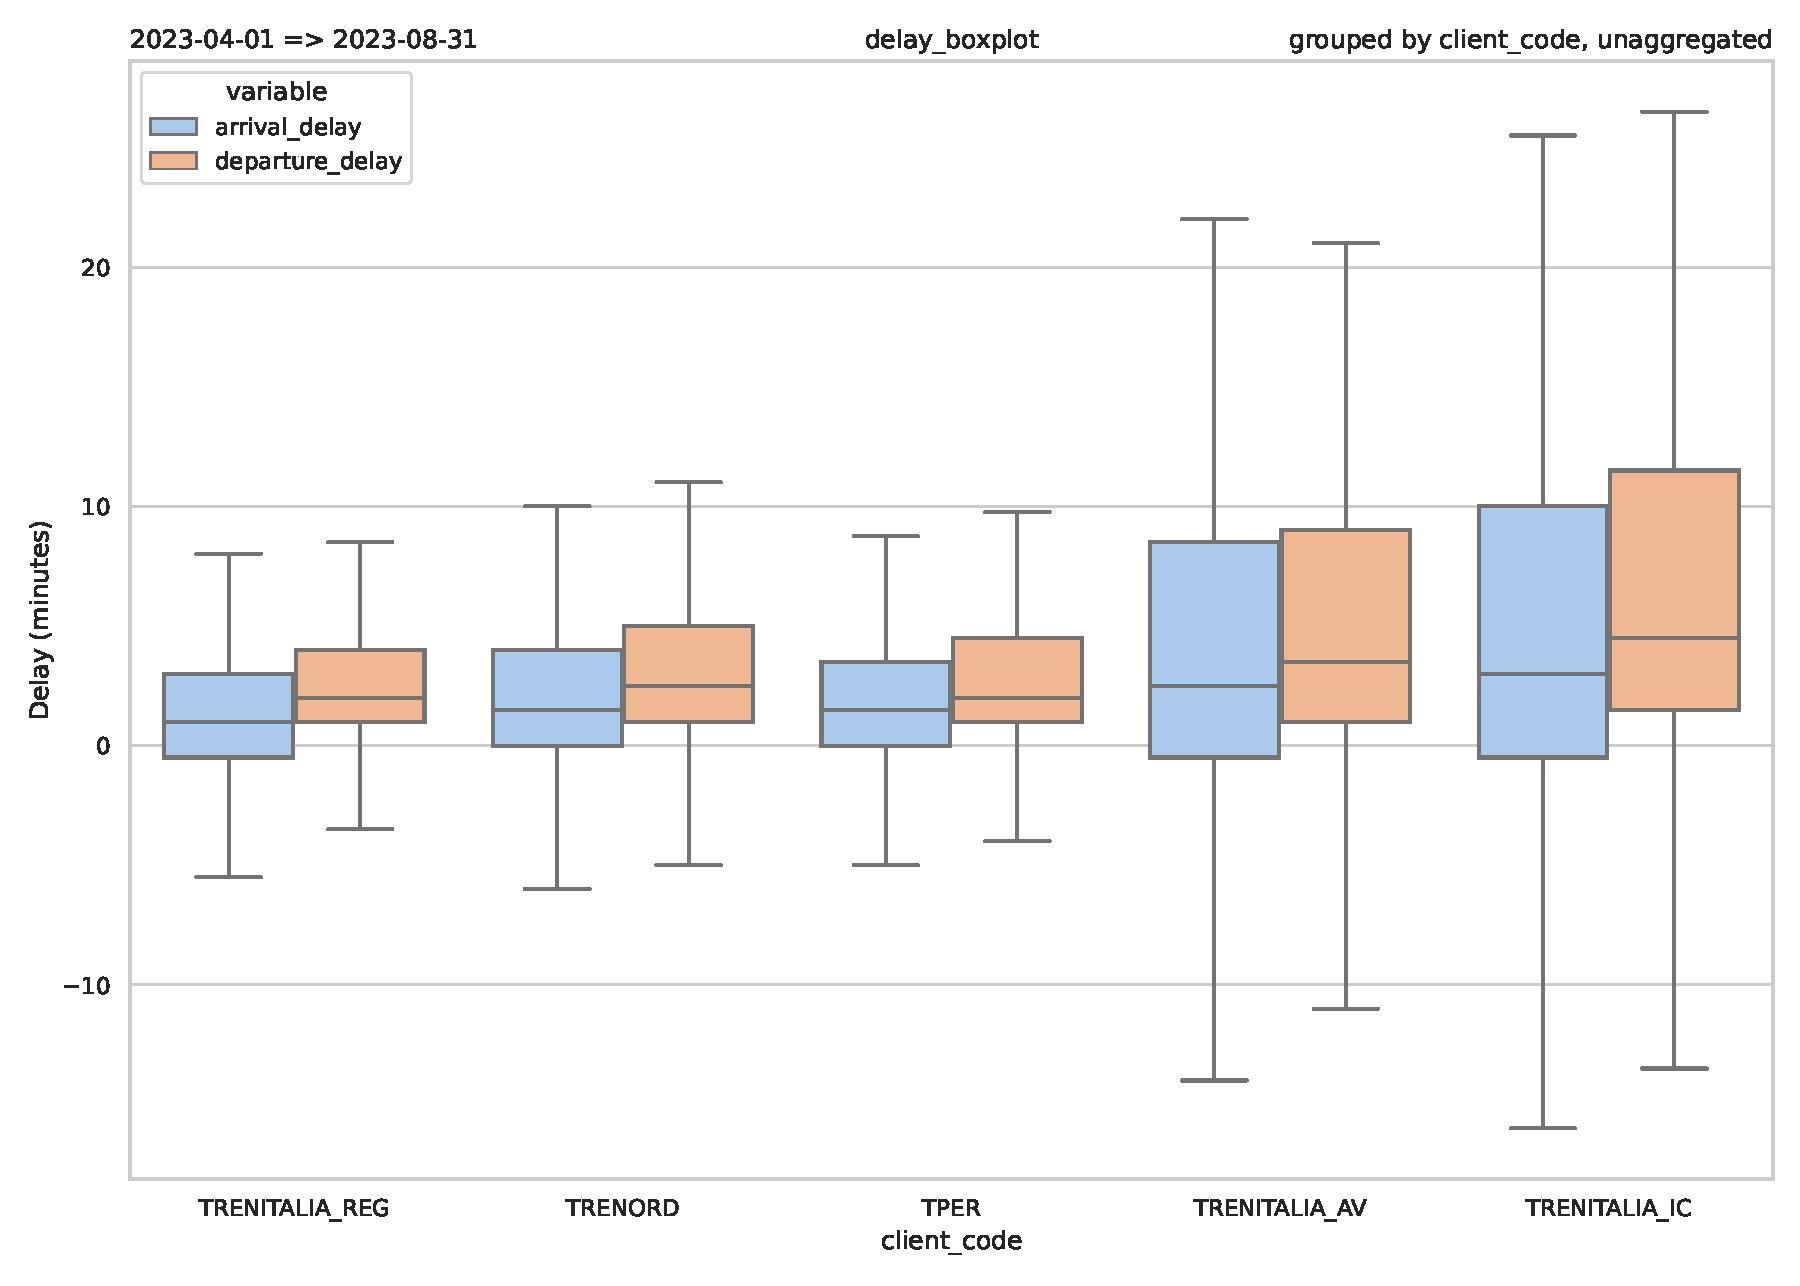
\includegraphics[width=0.96\textwidth]{images/delay_box_rc.pdf}
    \caption{Boxplot dei ritardi, raggruppato per impresa ferroviaria}
    \label{figure:delay_box_rc}
\end{figure}

L'ultima visualizzazione predefinita, \texttt{trajectories\_map}, apre
sul browser una \textbf{mappa temporizzata} della circolazione
ferroviaria.  Ogni treno è rappresentanto da una \textbf{linea
    colorata} avente come \textit{testa} un poligono indicante la
categoria posizionato nella fermata attuale.

\subsection*{Altre statistiche}

La \textbf{forte versalità} del formato CSV permette facilmente di
eseguire \textbf{ulteriori analisi}, anche senza utilizzare
l'\textit{analyzer}.  Nell'Elaborato (vedi \S~3.2) sono state proposte
altre analisi, come quella in \figurename~\ref{figure:intraday}.

\begin{figure}[h]
    \centering
    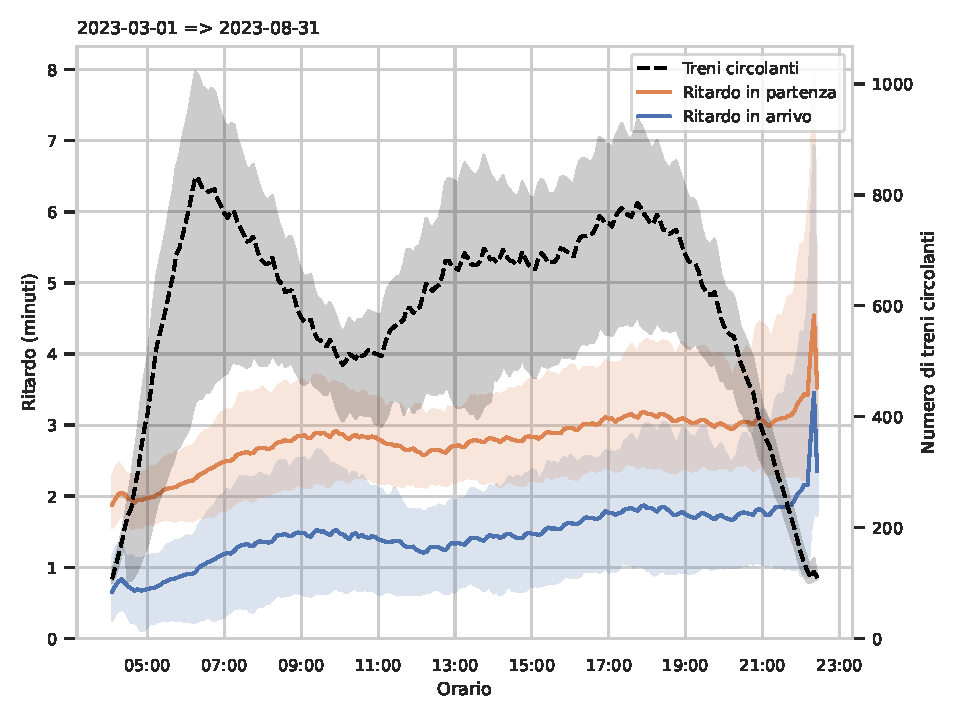
\includegraphics[width=0.95\textwidth]{images/intraday_delay.pdf}
    \caption{Andamento del ritardo infragiornaliero nei mesi considerati}
    \label{figure:intraday}
\end{figure}

\section{Conclusioni}

L'\textbf{obiettivo principale} del progetto è stato raggiunto: è ora
disponibile a \textit{chiunque} uno strumento adibito alla produzione
di \textit{dataset} di alta qualità sulla \textit{performance} della
circolazione ferroviaria italiana.  Gli \textbf{aspetti legali} sono
ancora oggetto di discussione: studi futuri potranno approfondire il
ruolo della \textbf{trasparenza} delle partecipate operanti in un
contesto di servizio pubblico.

\end{document}
%%% Local Variables:
%%% mode: latex
%%% TeX-master: t
%%% End:
